\documentclass[a4paper,10pt]{article}

\usepackage[english]{babel}
\usepackage{graphicx}
\usepackage[colorlinks, linkcolor=black, citecolor=black, urlcolor=black]{hyperref}
\usepackage{geometry}
\usepackage{xspace} 
\geometry{tmargin=3cm, bmargin=2.2cm, lmargin=2.2cm, rmargin=2cm}
\usepackage{todonotes} %Used for the figure placeholders

\newcommand\todoin[2][]{\todo[inline, caption={2do}, #1]{
\begin{minipage}{\textwidth-4pt}#2\end{minipage}}}

\newcommand{\rem}{\emph{ReMeS}\xspace}

% Your name and student number must be filled in on the title page found in
% titlepage.tex.

\begin{document}
\begin{titlepage}
    \newpage
    \thispagestyle{empty}
    \frenchspacing
    \hspace{-0.2cm}
    \includegraphics[height=3.4cm]{sedes}
    \hspace{0.2cm}
    \rule{0.5pt}{3.4cm}
    \hspace{0.2cm}
    \begin{minipage}[b]{8cm}
        \Large{Katholieke\newline Universiteit\newline Leuven}\smallskip\newline
        \large{}\smallskip\newline
        \textbf{Departement\newline Computerwetenschappen}\smallskip
    \end{minipage}
    \hspace{\stretch{1}}
    \vspace*{3.2cm}\vfill
    \begin{center}
        \begin{minipage}[t]{\textwidth}
            \begin{center}
	            \LARGE{\rm{\textbf{\uppercase{Remote Measurement, Monitoring
                    and Control System}}\\The complete architecture}}\\
                \Large{\rm{Software Architecture (H09B5a) - Part 2b}}
            \end{center}
        \end{minipage}
    \end{center}
    \vfill
    \hfill\makebox[8.5cm][l]{%
        \vbox to 7cm{\vfill\noindent
            {\rm \textbf{Toon Nolten (r0258654)}}\\
            {\rm \textbf{Nele Rober (r0262954)}}\\[2mm]
            {\rm Academic year 2013-2014}
        }
    }
\end{titlepage}


\tableofcontents
\listoffigures
\newpage

\section{Introduction}\label{sec:introduction}
The architecture satisfies all non-functional requirements while kept as simple as possible. This results in an architecture that allows for an easy division of the implementation of the subsystems across fairly independent business units. It also allows the investers to minise their risk by implementing the system in a modular fashion, thereby testing the waters to see if people are interested in the services \rem offers.

\section{Overview}\label{sec:overview}
\subsection{Architectural decisions}

\paragraph{\emph{Av2}: Missing Measurements}
\rem should be able to detect missing measurements. This responsability is assigned to a MeasurementArrivalMonitor. All RMM-\rem communication passes through the RMMFacade and is acknowledged. Availability of communication is very important, therefore a CommunicationAvailabilityMonitor is added to the RMMCommunication.

\paragraph{\emph{Av3}: Third Party Billing Service Failure}
To improve reliability of communication between \rem and third parties a ThirdPartyCommunication is added. This component is used to make sure that invoices either arrive at the Third Party Billing Service or an operator is notified.

\paragraph{\emph{P2}: Anomaly Detection}
To enable performant anomaly detection, the AnomalyScheduler identifies when to go to overloaded modus and will then schedule incoming measurements appropriately. Multiple instances of MeasurementProcessors and AlarmValidator allow to process any number trames within the required deadline.

\paragraph{\emph{P3}: Requests to the Measurement Database}
When in overloaded modus, the system should go back to normal modus as soon as possible while giving priority to premium service level customers. A scheduler is necessary to accomplish this.

\paragraph{\emph{M2}: Fine-grained Metering for Enterprises}
The CustomerDB knows who should pay for the measurements and who should be paid. This allows an easy modification of the Billing component when secondary RMMs are added.

\paragraph{\emph{M3}: Decentralized Electricity Generation}
The CustomerDB knows who should pay for the measurements and who should be paid. This allows an easy modification of the Billing component when RMMs that measure production of electricity are added.


\subsection{Discussion}

\paragraph{Responsibilities}
Every service of \rem is provided by a different component. This makes it possible to implement and maintain each service independently, allowing responsibility for subsystems to be delegated to individual business entities with a minimum of interdependence.

Another benefit of this clear separation lies in the fact that \rem can be bootstrapped in a modular fashion. Provided the core functionalities are available (i.e. receiving measurements, storing measurements and making them available to our customers), \rem can start functioning (as a pilot project: generating valuable feedback early) and add other functionality incrementally. This decreases the initial investment and associated risk, making the project more attractive from a business standpoint.

Lastly it allows for graceful degradation of the system: a failure of the billing subservice does not influence unrelated functionality.
Even when the communication with RMMs fails, users can still consult an overview of measurements up to the failure.

\paragraph{Coupling}
The databases are highly coupled with other components of \rem. However the customer database is often only needed in case a subsystem is overloaded: only then its scheduler needs the SLAs to infer the priority. In the current architecture the SLAs have to be cached, to avoid shifting the load to the customer database. 

In retrospect we might have better distributed the data over more databases, e.g. separate information regarding devices from information regarding customers, providing a seperate database for SLAs, etc.

\paragraph{Security}
Having a single component responsible for most of the communication with the outside world reduces the attack surface of \rem. This makes it easier to focus security related development.

Currently a user is identified by a secret token he receives when logging in. However, because of lack of knowledge, we are not sure this is a proper way of securing the communication. We did not focus on improving this aspect of the architecture because there were no security related non-functional requirements.

\section{Context}\label{sec:context}
External components can communicate with \rem through three components: RMMCommunication, ThirdPartyCommunication and NotificationHandler.
All communication between \rem and RMMs goes through the RMMCommunication, e.g. reporting measurements and alarms, configuring and actuating modules.

All communication with third parties is handled by the ThirdPartyCommunication and the NotificationHandler. The first provides `online' communication, the second `offline' communication, e.g. regular mail, SMS, etc.
The ThirdPartyCommunication communicates with all kinds of interfaces, for example an online web client for customers, the UIS.

Figure \ref{fig:cc-context} illustrates these three components and the interfaces offered to third parties.
The following interfaces are considerd:
\begin{itemize}
	\item \emph{UtilityInformationSystem:} The interface provided by the utility company.
    \item \emph{ThirdPartyBillingService:} The interface provided by an external service that handles the sending of invoices and the following up of payments.
    \item \emph{UserInterface:} A web interface that a user (customer and technician) can use to communicate with \rem.
    \item \emph{CallCenter:} A web interface that a CallCenter operator can use to communicate with \rem.
    \item \emph{PostalServce:} The interface provided by an external service that sends regular mail for \rem.
    \item \emph{SMSService:} The interface provided by an external service that sends text messages (sms) for \rem.
    \item \emph{EmailService:} The interface provided by an external service that e-mail for \rem.
    \item \emph{RemoteModule:} The interface provided by an RMM. All communication goes via trames.
    \item \emph{RemoteActuator:} The interface provided by a remote actuator. All communication goes via trames.
\end{itemize}


\begin{figure}[!htp]
    \centering
    \includegraphics[width=\textwidth]{Context_ Main}
    \caption{Context diagram for \rem.
        }\label{fig:cc-context}
\end{figure}

\section{Architectural overview}\label{sec:main-decomposition}
\rem provides several services: collection and storage of measurements, anomaly detection, billing, etc.
Each of these services is provided by a different component (respectively RMMCommunication, MeasurementDBManager, AnomalyDetector, Billling, etc.), figure \ref{fig:cc-primary}.

\begin{figure}[!htp]
    \centering
    \includegraphics[width=\textwidth]{Main Component Diagram}
    \caption{Main components}\label{fig:cc-primary}
\end{figure}

\subsection{Main architectural decisions}

\subsubsection{\emph{Av2}: Missing Measurements}

\paragraph{Design} figure \ref{fig:dec_rmmcomm}

\begin{enumerate}
	\item The MeasurementArrivalMonitor can detect missing meaurements by comparing the elapsed time with the expected arrival time of a trame. The expected time is calculated from the arrival time of the last trame of that RMM and the scheduled trame frequency.
    \item All communication between RMMs and \rem passes through and is acknowledged by the RMMFacade.
    \item The CommunicationAvailabilityMonitor regulary pings the Communication components and notifies an operator when one of them does not respond.
    \item When the communication channel fails, the MeasurementArrivalMonitor keeps track of how long the failure remains.
\end{enumerate}

\begin{figure}[!htp]
    \centering
    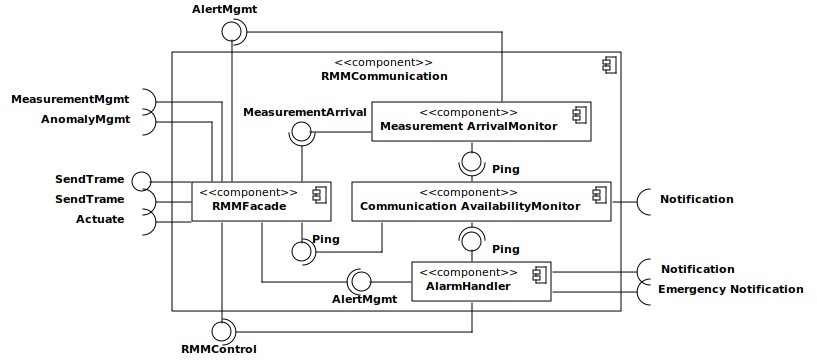
\includegraphics[width=\textwidth]{Decomposition_ Communication with RMM}
    \caption{Decomposition of the \texttt{RMMCommunication}}\label{fig:dec_rmmcomm}
\end{figure}

\noindent Tactics and patterns used:
\begin{itemize}
	\item Ping-echo
    \item Facade
\end{itemize}

\paragraph{Rationale} Alarms are irrelevant for the detection of missing measurements so a RMMFacade forwards only incoming measurements to the MeasurementArrivalMonitor. To minimise the load on the RMMFacade, the checking for missing measurements is done by a seperate component: the MeasurementArrivalMonitor. Detecting failures should happen on a different component than the component to check. The CommunicationAvailabilityMonitor is created for this purpose. Other Communication components can be monitored with it later on.

\paragraph{Alternative for the CommunicationAvailabilityMonitor} The components of the Communication subsystem could be checked for availability by other components of the Communication subsystem, for example, the Alarm Handler could check the MeasurementArrivalMonitor. However, all components would have to know how to notify the operators and all components would have to run on different machines so this would be less flexible than the CommunicationAvailabilityMonitor.

\paragraph{Alternative for the RMMFacade} The RMMs could send measurements and alarms to different receivers, but this complicates communication to and from RMMs.


\subsubsection{\emph{Av3}: Third Party Billing Service Failure}

\paragraph{Design} figure \ref{fig:dec_thirdparty}

\begin{enumerate}
	\item Every request to the Third Party Billing Service is acknowledged to the ThirdPartyCommunication component.
    \item The ThirdPartyCommunication component caches all billing requests untill they are acknowledged.
    \item When the ThirdPartyCommunication component does not reveice an acknowledgement in time, the request is resent in a proper fashion, e.g. exponential backoff.
    \item The ThirdPartyCommunication keeps track of the number of times a request is sent but not acknowledged and notifies an operator when this happens five times.
\end{enumerate}

\begin{figure}[!htp]
    \centering
    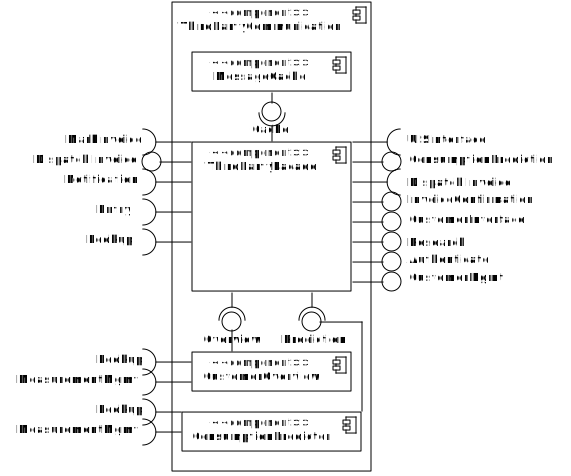
\includegraphics[width=\textwidth]{Decomposition_ Communication with third parties}
    \caption{Decomposition of the \texttt{ThirdPartyCommunication}}\label{fig:dec_thirdparty}
\end{figure}

\noindent Tactics and patterns used:
\begin{itemize}
	\item Facade
\end{itemize}

\paragraph{Rationale} Availability of third party components may not be limited to the Third Party Billing Service: other third parties may also require some kind of action when they become unavailable. Therefore the ThirdPartyCommunication is assigned this task.

\paragraph{Alternative for availability in the ThirdPartyCommunication}
The Billing component may handle the resending of unacknowledged requests itself, but then it would not be possible to reuse this functionality for other components that communicate with third parties.

\subsubsection{\emph{P2}: Anomaly Detection}

\paragraph{Design} figures \ref{fig:dec_anomaly} and \ref{fig:dec_alarmhandler}

\begin{enumerate}
    \item In normal modus, the AnomalyScheduler forwards the incoming measurements in first-in, first-out order. Alarms are handled before measurements and scheduled based on priority.
    \item In overloaded modus, the AnomalyScheduler forwards the incoming measurements by prioritising based on the SLA. Alarms are handled before measurements, but only when this does not endanger the individual deadline of measurements.
    \item Based on the load multiple instances of components other than the AnomalyScheduler can be added.
    \item The AnomalyScheduler can detect when it is necessary to go into overloaded modus.
    \item Alarms that come from an RMM are checked for validity by the AlarmValidator.
    \item High priority alarms from an RMM are sent to the AlarmHandler as well as the AnomalyDetector. When the alarm does not appear to be valid, the AlarmHandler is notified to cancel/undo the handling of the alarm.
    \item The AlarmValidator can keep track of wich RMMs sends invalid alarms to \rem and can notify the operators when one of the RMMs ferquently sends false alarms.
   	\item The AlarmValidator can ask an RMM for more measurements via the RMMFacade.
\end{enumerate}

\begin{figure}[!htp]
    \centering
    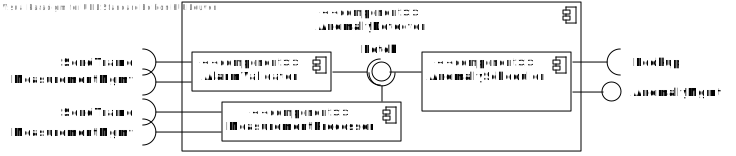
\includegraphics[width=\textwidth]{Decomposition_ AnomalyDetector}
    \caption{Decomposition of the \texttt{AnomalyDetector}}\label{fig:dec_anomaly}
\end{figure}

\begin{figure}[!htp]
    \centering
    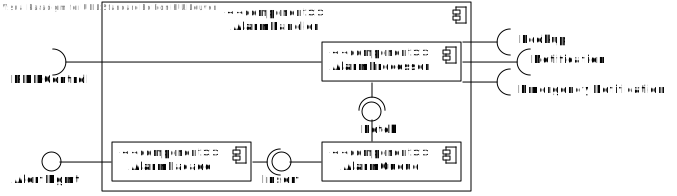
\includegraphics[width=\textwidth]{Decomposition_ AlarmHandler component}
    \caption{Decomposition of the \texttt{AlarmHandler}}\label{fig:dec_alarmhandler}
\end{figure}

\noindent Tactics and patterns used:
\begin{itemize}
	\item Scheduler
\end{itemize}

\paragraph{Rationale} In overloaded modus, it is required to schedule the processing by SLA, so an AnomalyScheduler is in order. Alarms that are generated by RMMs may not be reliable because RMMs do not have a lot of resources to ensure validity of alarms. When an RMM malfunctions and keeps sending invalid alarms, the AlarmValidator can notice this, notify operators via RMMCommunication and shut off the device if necessary. Some anomalies may not be recognised by an RMM, because more knowledge is required. The MeasurementProcessor can detect these anomalies.

\paragraph{Alternative for the AlarmValidator}
Assuming that RMMs send only valid alarms, an AlarmValidator is not necessary and will slow the alarm handling down. However, if an RMM malfunctions and floods \rem with alarm notifications, this may block everything else. The AlarmValidator avoids this.

\subsubsection{\emph{P3}: Requests to the measurement database}

\paragraph{Design} figure \ref{fig:dec_measurement}

\begin{enumerate}
	\item The MeasurementManager receives all incoming requests and sends all outgoing replies to the appropriate recipient.
	\item In normal modus, the RequestScheduler schedules the incoming requests in FIFO order.
    \item If the system fails to comply to the specified deadlines, the MeasurementManager will notice this and activates the RequestScheduler's overloaded modus.
    \item To make sure that requests can be scheduled approriately, the MeasurementManager adds the SLA to the request before handing it over to the RequestScheduler.
    \item In overloaded modus, the RequestScheduler schedules requests in the order that returns the system to normal modus the fastest, giving precedence to premium service level customers and history queries that are used for anomaly detection.
    \item In overloaded modus, the ReplicaManager may return a stale cached anwser to history queries.
\end{enumerate}

\begin{figure}[!htp]
    \centering
    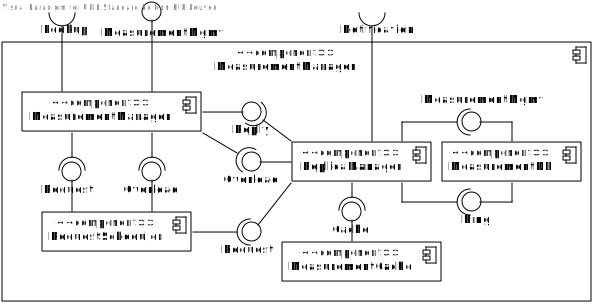
\includegraphics[width=\textwidth]{Decomposition_ MeasurementDBManager}
    \caption{Decomposition of the \texttt{MeasurementDBManager}}\label{fig:dec_measurement}
\end{figure}

\noindent Tactics and patterns used:
\begin{itemize}
	\item Scheduler
\end{itemize}

\paragraph{Rationale} The RequestScheduler is necessary to determine the order of requests in overloaded modus. To avoid that the RequestScheduler is bothered with outgoing replies, the MeasurementManager is added.

\paragraph{Alternative for the MeasurementManager} The MeasurementManager is not strictly necessary: the RequestScheduler could send the replies to the appropriate recipients and measure the times to process requests to decide when to go into overloaded modus. However, the RequestScheduler should not be bothered with things other than scheduling.


\subsubsection{\emph{M2}: Fine-grained metering for enterprises}

\paragraph{Design}

\begin{enumerate}
	\item The CustomerDB keeps track of who pays for and who receives payment for a utility measured by an RMM. If these are undefined the RMM is considered a secondary RMM.
    \item The Billing component will only take into account consumption measured by primary RMMs.
\end{enumerate}

\paragraph{Rationale}
The sole difference between primary and secondary RMMs is that only consumption measured by primary RMMs is billed. So only the Billing component has to know there is a difference.


\subsubsection{\emph{M3}: Decentralized Electricity Generation}

\paragraph{Design}

\begin{enumerate}
	\item A customer who produces electricity should have two RMMs (this may be one device with two IDs): one for produced electricity and one for consumed electricity.
    \item The CustomerDB knows who pays for and who receives payment for the utility measured by each RMM.
    \item The Billing component uses this information to retrieve every RMM ID for which a customer should be billed. The Billing component has access to the MeasurementDBManager to retrieve the relevant measurements.
\end{enumerate}

\paragraph{Rationale} To be able to distinguish between consumed and produced electricty two RMM IDs are used. The Billing component should know who should be billed and who that person should pay, therefore two fields are stored in the CustomerDB. Keeping two fields increases flexibility: in the future it might be possible that person A pays person B, without any Utility Company in between or \rem might offer RMMs that measure things that don't need to be billed (e.g. temperature, chemicals...), a customer then `pays himself'.

\paragraph{Alternatives for the two fields in the CustomerDB}
A trame could contain a field that indicates whether it measures consumption or production. However, this addition in functionality would require a change in the MeasurementDB schema and is less flexible than the current solution.

It is possible to store a Billing Type in the CustomerDB instead of two fields: positive billing (consumed), negative billing (produced) and no billing. However, this solution does not make it possible to let person A provide a utility to person B without the intervention of a Utility Company (e.g. a chemical plant that supplies another plant with its products).

\section{Deployment view}\label{sec:deployment}
Communication with RMM has to be simple (for the module) and allow for alternative channels (like SMS), therefore we chose UDP.
Communication with most third parties relies on tcp for reliability, the communication with the users and possibly the callcenter would be based on an html interface, figure \ref{fig:depl_context}.

\begin{figure}[!htp]
    \centering
    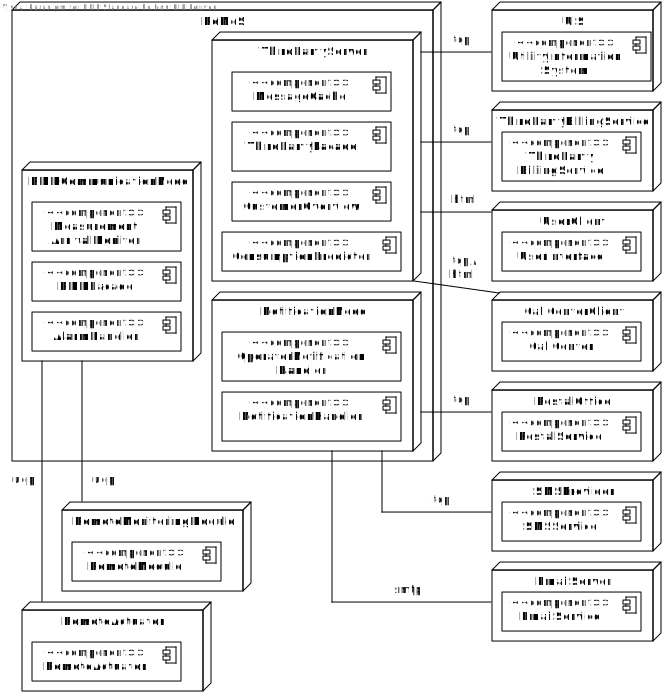
\includegraphics[width=\textwidth]{Context}
    \caption{Context diagram for the deployment view.}\label{fig:depl_context}
\end{figure}

Figure \ref{fig:depl_primary}, shows our deployment.
There are three measurement database nodes, as long as each node has an availability of 90\% or more, the total availability will be 99.9\%. The CustomerOverview and Consumption predictions could be run on a seperate node but since we do not expect a high load from third party communication this is not yet necessary. Most components run on a node together with the other components they are closely related to, except for the availability monitor which needs to be on a separate node and the alarmhandler which is a critical subsystem relied on by multiple parts of \rem.

\begin{figure}[!htp]
    \centering
    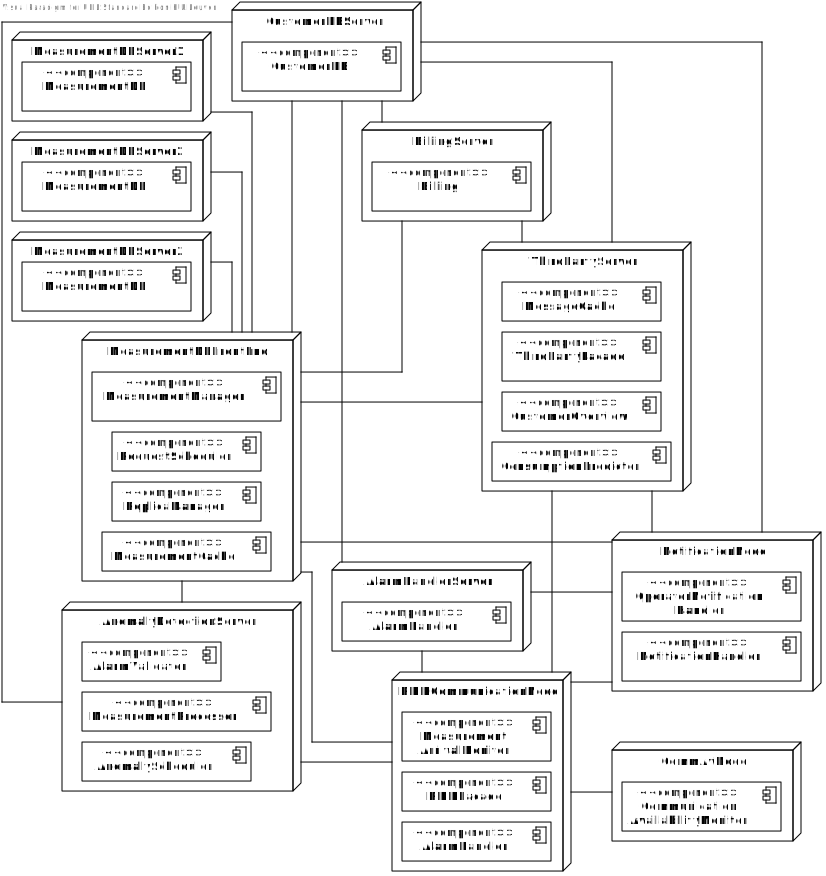
\includegraphics[width=\textwidth]{Deployment Diagram}
    \caption{Diagram for the deployment view.}\label{fig:depl_primary}
\end{figure}

\section{Scenarios}\label{sec:scenarios}

\subsection{User profile creation}
Customers can register in two ways: via the CallCenter and through the online interface.
In the first case (fig. \ref{fiq:seq_registration1}) a CallCenter Operator initiates the registration and asks the customer for the required information.
When all required information is acquired the CallCenter Operator goes over the information with the customer to verify and then confirms the registration.

In the second case (fig. \ref{fiq:seq_registration2}) the customer iniates the registration online and enters the required information which is stored by \rem as a tentative registration.
A CallCenter Operator then goes over the information and approves the registration.
Then the customer is sent a unique registration identifier via regular mail, which he can use to confirm the registration to \rem.

After confirmation the customer's profile is permanently stored in the CustomerDB and ready to be associated with devices.
A technician is also scheduled to install one or more new devices.

\begin{figure}[!htp]
    \centering
    \includegraphics[width=\textwidth]{Registration_ CallCenter}
    \caption{Customer registration through the CallCenter.}
    \label{fig:seq_registration1}
\end{figure}

\begin{figure}[!htp]
    \centering
    \includegraphics[width=\textwidth]{Registration_ Customer}
    \caption{Customer registration through the online interface.}
    \label{fig:seq_registration2}
\end{figure}

\subsection{User profile association with a remote monitoring module}
After installing a RMM the technician notifies \rem, \rem then updates the customer's information and notifies the UIS (fig. \ref{fiq:seq_association}).

\begin{figure}[!htp]
    \centering
    \includegraphics[width=\textwidth]{User profile association with a remote monitoring module}
    \caption{Device association with a customer.
        }\label{fig:seq_association}
\end{figure}

\subsection{Transmission frequency reconfiguration}
The customer indicates via the online interface that he wants to change the transmission frequency of one of his devices through the ThirdPartyCommunication. This change to the configuration is checked and then communicated to the RMM through the RMMCommunication.

\subsection{Troubleshooting}
When remote monitoring modules malfunction the \rem operators are notified, they try to resolve the problem and conctact the customer for onsite troubleshooting if necessary. If the customer indicates he cannot resolve the problem a technician is scheduled to repair/replace the device.

\subsection{Alarm notification recipient configuration}
The customer accesses his overview by logging in to the online interface. Here he can add, remove and edit alarm recipients for each of his devices. Each recipient is asked to confirm their willingness to receive alarm notifications. The ThirdPartyCommunication then updates the DeviceInformation stored in the CustomerDB.

\subsection{Remote control}
After logging in to the online interface a customer has the options to control a device directly or to alter the device's configuration which may cause the device to actuate the corresponding actuator.

\subsection{Normal measurement data transmission}
The RMM sends a measurement to \rem through the RMMFacade (fig. \ref{fig:seq_measurement}). The RMMFacade forwards this measurement to the MeasurementDBManager, the MeasurementArrivalMonitor and the AnomalyDetector where it is checked for anomalies (cf. Alarm data transmission: \rem).

\begin{figure}[!htp]
    \centering
    \includegraphics[width=\textwidth]{RMM Transmission}
    \caption{Incoming Measurement.}
    \label{fig:seq_measurement}
\end{figure}

When a measurement is lost or an RMM does not send a measurement (fig. \ref{fiq:seq_missed}), this is noticed by the MeasurementArrivalMonitor which notifies the \rem operators and the alarm recipient of the problem.

\begin{figure}[!htp]
    \centering
    \includegraphics[width=\textwidth]{Missing measurement}
    \caption{Missing measurement.}
    \label{fig:seq_missed}
\end{figure}

\subsection{Individual data analysis}
All incoming measurements are forwarded to the AnomalyDetector (fig. \ref{fig:seq_measurement}) to be compared to historical consumption so as to detect anomalous measurements.

\subsection{Utility production planning analysis}
The ConsumptionPredictor regularly analyses the stored measurements to be able to forecast future demand. The Utility Information System can access predictions for his customer base through the ThirdPartyCommunication.

\subsection{Information exchange towards the UIS}
\rem utilizes the UISInterface to request current pricing information and to notify the utility company of new customers or customers who have cancelled their subscription.

\subsection{Alarm data transmission: remote monitoring module}
When an RMM detects an anomaly it sends an AlarmTrame to the RMMFacade (fig. \ref{fig:seq_alarm}). How an alarm is handled depends on its priority. High priority alarms, i.e. gas alarms, are immediately sent to the AlarmHandler which resolves the alarm by actuating appropriate actuators and notifying alarm recipients and the Emergency Services. Furthermore the alarm is also sent to the AnomalyDetector which can request further measurements from the RMM to validate the alarm. If the alarm turns out not to be valid the AlarmHandler is requested, through the RMMFacade, to cancel the alarm by cancelling the handling of the alarm, sending a notfication that the alarm was a false alarm and restoring the state of all actuators that were influenced by the alarm.

Low priority alarms are first sent to the AnomalyDetector for validation. If the alarm is considered valid the AnomalyDetector will contact the AlarmHandler through the RMMFacade. The AlarmHandler actuates the appropriate actuators and notifies all alarm recipients.

\begin{figure}[!htp]
    \centering
    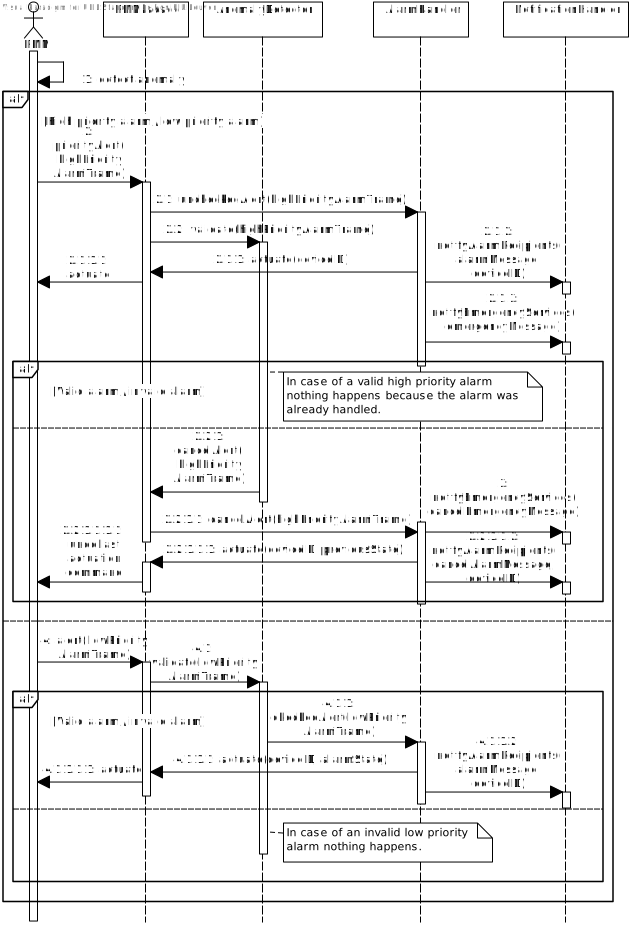
\includegraphics[width=\textwidth]{RMM Alarm}
    \caption{An alarm from an RMM reaches \rem.}
    \label{fig:seq_alarm}
\end{figure}

\subsection{Alarm data transmission: \rem}
The AnomalyDetector detects an anomaly in the measurements (fig. \ref{fig:seq_measurement}) of an RMM that was not noticed by the RMM itself. It notifies the AlarmHandler through the RMMFacade. The AlarmHandler handles the alarm appropriately: in accordance with the customers profile.

\subsection{Low battery alarm}
The RMM sends a trame containing its PowerStatus. The RMMFacade passes this to the AlarmHandler which passes it to the NotificationHandler to be delivered to the customer. The customer can then replace the battery or contact the CallCenter to troubleshoot his device.

\subsection{Remote control module de-activation}
The customer indicates he wants to de-activate a device, the device is then reconfigured not to send any more measurements and is removed from the customer's account.

\subsection{New bill creation}
The Billing component decides an Invoice should be generated for a certain customer, it then contacts the ThirdPartyBillingService and the UIS through the ThirdPartyCommunication.

\subsection{Bill payment is received}
The ThirdPartyBillingService contacs \rem via the ThirdPartyCommunication which tells the Billing component to mark the invoice paid.

\appendix
\section{Element catalog}\label{app:catalog}

\subsection{AnomalyDetector}
\paragraph{Responsabilities} 
The AnomalyDetector
\begin{itemize}
    \item Detects anomalies in the measurements;
    \item Validates alarms from RMMs;
    \item Detects when an RMM keeps sending invalid alarms;
\end{itemize}

\paragraph{Super component} \rem

\paragraph{Sub components} AlarmValidator, AnomalyScheduler, MeasurementProcessor

\paragraph{Provided interfaces}
\begin{itemize}
	\item AnomalyMgmt
\end{itemize}

\subsection{AnomalyScheduler}
\paragraph{Responsabilities} 
The AnomalyScheduler
\begin{itemize}
	\item Schedules incoming anomaly detection and validation request;
    \item Determines when to go to overload modus;
\end{itemize}

\paragraph{Super component} AnomalyDetector

\paragraph{Sub components} None

\paragraph{Provided interfaces}
\begin{itemize}
	\item AnomalyMgmt
    \begin{itemize}
    	\item \texttt{void detectAnomaly(MeasurementTrame measurement)}
        \begin{itemize}
        	\item Effect: The measurement is checked upon anomalies.
            \item Exceptions: None
        \end{itemize}
        \item \texttt{void validate(AlarmTrame alarm)}
        \begin{itemize}
            \item Effect: The alarm is validated.
            \item Exceptions: None
		\end{itemize}
    \end{itemize}
    \item Fetch
    \begin{itemize}
    	\item \texttt{MeasurementTrame fetchMeasurement()}
        \begin{itemize}
        	\item Effect: A measurement is returned.
            \item Excsptions: None
        \end{itemize}
        \item \texttt{AlarmTrame fetchAlarm()}
        \begin{itemize}
        	\item Effect: An alarm is returned.
            \item Excsptions: None
        \end{itemize}
    \end{itemize}
\end{itemize}

\subsection{AlarmFacade}
cf. assignment

\subsection{AlarmHandler}
\paragraph{Responsabilities} 
The AlarmHandler
\begin{itemize}
	\item Receives incoming alarms;
    \item Notifies the NotificiationHandler when nessecary;
    \item Activates the actuators when nessecary;
\end{itemize}

\paragraph{Super component} RMMCommunication

\paragraph{Sub components} None

\paragraph{Provided interfaces}
\begin{itemize}
	\item AlertMgmt
    \begin{itemize}
    	\item \texttt{void anomalyDetectedAlert(AlarmTrame alarm}
        \begin{itemize}
            \item Effect: The alarm is handled by actuating appropriate actuators and notifying the NotificationHandler. This method is called for anomalies detected by the AnomalyDetector.
            \item Exceptions: None
		\end{itemize}
    	
    	\item \texttt{void cancelAlert(AlarmTrame highPriorityAlarm)}
        \begin{itemize}
            \item Effect: The alarm is canceled. This happens when the AlarmHandler was asked to handle a high priority alert that was later noticed to be invalid by the AnomalyDetector.
            \item Exceptions: None
        \end{itemize}
        \item \texttt{void checkedAlert(AlarmTrame lowPriorityAlarm)}
        \begin{itemize}
            \item Effect: The alarm is acknowledged and handled. This method is called after low priority alarms are validated by the AnomalyDetector.
            \item Exceptions: None
		\end{itemize}
        
        \item \texttt{void lowBatteryAlert(DeviceID device, PowerStatus status) throws NoSuchDeviceException}
        \begin{itemize}
        	\item Effect: The customer is notified of the low power status of the RMM.
            \item Exceptions:
            \begin{itemize}
                \item NoSuchDeviceException: Thrown when the given device does not exist.
            \end{itemize}
        \end{itemize}
        
        \item \texttt{void notifyDeviceMalfunction(DeviceID device, AlarmMessage alarm) throws NoSuchDeviceException}
        \begin{itemize}
            \item Effect: A \rem operator is notified of a malfunctioning device, e.g. many false alarms, sporadic communication, etc.
            \item Exceptions:
            \begin{itemize}
                \item NoSuchDeviceException: Thrown when the given device does not exist.
            \end{itemize}
		\end{itemize}
        
        \item \texttt{void notifyMissingMeasurement(DeviceID device, AlarmMessage alarm) throws NoSuchDeviceException}
        \begin{itemize}
            \item Effect: A \rem operator is notified of a missing measurement.
            \item Exceptions:
            \begin{itemize}
                \item NoSuchDeviceException: Thrown when the given device does not exist.
            \end{itemize}
		\end{itemize}
        
        \item \texttt{void uncheckedAlert(AlarmTrame highPriorityAlarm)}
    	\begin{itemize}
            \item Effect: The alarm is handled by actuating appropriate actuators and notifying the NotificationHandler. This method is called for urgent, unchecked alerts.
            \item Exceptions: None
		\end{itemize}
    \end{itemize}
    
	\item Ping
\end{itemize}

\subsection{AlarmProcessor}
cf. assignment

\subsection{AlarmQueue}
cf. assignment

\subsection{AlarmValidator}
\paragraph{Responsabilities} 
The AlarmValidator
\begin{itemize}
	\item Checks the validity of alarms from RMMs;
    \item If a lot of invalid alarms from a certain RMM arrive, the operators are notified;
\end{itemize}

\paragraph{Super component} AnomalyDetector 

\paragraph{Sub components} None

\subsection{Billing}
\paragraph{Responsabilities} 
The Billing component
\begin{itemize}
	\item Generates invoices, determining its schedule on the billing information of customers;
    \item Saves all sent invoices (in an internal database);
\end{itemize}

\paragraph{Super component} \rem

\paragraph{Sub components} None

\paragraph{Provided interface}
\begin{itemize}
	\item MarkInvoice
    \begin{itemize}
    	\item \texttt{void markInvoicePaid(InvoiceID invoice) throws NoSuchInvoiceException}
        \begin{itemize}
        	\item Effect: Marks the invoice as paid.
            \item Exceptions:
            \begin{itemize}
            	\item NoSuchInvoiceException: Thrown when the given invoice does not exist.
            \end{itemize}
        \end{itemize}
    \end{itemize}
\end{itemize}

\subsection{CommunicationAvailabilityMonitor}
\paragraph{Responsabilities} 
The CommunicationAvailabilityMonitor
\begin{itemize}
	\item Monitors the availability of the RMMCommunication subsystem components with pings;
    \item Notifies the operators when one of the internal components fails;
\end{itemize}

\paragraph{Super component} RMMCommunication

\paragraph{Sub components} None

\subsection{ConsumptionPredictor}
\paragraph{Responsabilities} 
The ConsumptionPredictor
\begin{itemize}
	\item Analyzes utility consumption patterns;
    \item Forecasts future consumption patterns;
\end{itemize}

\paragraph{Super component} ThirdPartyCommunication

\paragraph{Sub components} None

\paragraph{Provided interfaces}
\begin{itemize}
	\item Prediction
    \begin{itemize}
        \item \texttt{ConsumptionPrediction requestConsumptionPrediction(TimePeriod timePeriod) throws NoPredictionPossibleException}
        \begin{itemize}
        	\item Effect: Calculates the consumption prediction.
            \item Exception:
            \begin{itemize}
            	\item NoPredictionPossibleException: Throws when the request cannot be fulfilled.
            \end{itemize}
        \end{itemize}
    \end{itemize}
\end{itemize}

\subsection{CustomerDB}
\paragraph{Responsabilities} 
The CustomerDB
\begin{itemize}
	\item Stores all customer information;
    \item Stores which RMMs are associated to customers;
    \item Stores who pays for the measurements of each RMM and who receives payment;
    \item Stores the information relevant to billing;
    \item Stores the SLAs for each customer;
\end{itemize}

\paragraph{Super component} \rem

\paragraph{Sub components} None

\paragraph{Provided interfaces}
\begin{itemize}
	\item Entry
    \begin{itemize}
    	\item \texttt{void linkDevice(CustomerID customer, DeviceID device) throws NoSuchCustomerException, NoSuchDeviceException}
        \begin{itemize}
        	\item Effect: After a sanity check the given device and customer are linked.
            \item Exception:
           	\begin{itemize}
            	\item NoSuchCustomerException: Thrown when the given CustomerID is not associated with a customer.
                \item NoSuchDeviceException: Thrown when the given RMM does not exist.
            \end{itemize}
        \end{itemize}
        
    	\item \texttt{void removeCustomer(CustomerID customer) throws NoSuchCustomerException}
        	\begin{itemize}
            	\item Effect: The given customer is marked for removal.
                \item Exception:
                \begin{itemize}
                	\item NoSuchCustomerException: Thrown when the given CustomerID is not associated with a customer.
                \end{itemize}
            \end{itemize}
            
        \item \texttt{void removeDevice(DeviceID device) throws NoSuchDeviceException}
        \begin{itemize}
        	\item Effect: The given device is removed from the customer's account.
            \item Exception:
           	\begin{itemize}
                \item NoSuchDeviceException: Thrown when the given RMM does not exist.
            \end{itemize}
        \end{itemize}
    	\item \texttt{void storeCustomerInformation(CustomerInformation customerInfo)}
        	\begin{itemize}
            	\item Effect: The information is stored for the corresponding customer.
                \item Exceptions: None
            \end{itemize}
        \item \texttt{void storeDeviceInformation(DeviceInformation deviceInfo)}
        	\begin{itemize}
            	\item Effect: The information is stored for the corresponding RMM.
                \item Exceptions: None
            \end{itemize}
    \end{itemize}
    \item Lookup
    \begin{itemize}
    	\item \texttt{Collection<DeviceID> associatedDevices(CustomerID customer) throws NoSuchCustomerException}
        \begin{itemize}
            \item Effect: The DeviceIDs of devices  associated to the given customer are returned.
            \item Exceptions:
            \begin{itemize}
                \item NoSuchCustomerException: Thrown when the given customer does not exist.
            \end{itemize}
        \end{itemize}
   		\item \texttt{Collection<DeviceID> billedDevices(CustomerID customer) throws NoSuchCustomerException}
        \begin{itemize}
            \item Effect: The DeviceIDs for which the given customer should pay are returned.
            \item Exceptions:
            \begin{itemize}
                \item NoSuchCustomerException: Thrown when the given customer does not exist.
            \end{itemize}
        \end{itemize}
        \item \texttt{CustomerInformation customerInformation(CustomerID customer) throws NoSuchCustomerException}
        \begin{itemize}
            \item Effect: The information concerning the RMM is returned.
            \item Exceptions:
            \begin{itemize}
                \item NoSuchCustomerException: Thrown when the given customer does not exist.
            \end{itemize}
        \end{itemize}
        \item \texttt{DeviceInformation deviceInformation(DeviceID device) throws NoSuchRMMException}
        \begin{itemize}
            \item Effect: The information concerning the RMM is returned. This information includes the type of RMM, the alarmrecipients and the actuator that should handle alarms for this RMM.
            \item Exceptions:
            \begin{itemize}
                \item NoSuchDeviceException: Thrown when the given RMM does not exist.
            \end{itemize}
        \end{itemize}
        \item \texttt{SLA sla(CustomerID customer) throws NoSuchCustomerException}
        \begin{itemize}
            \item Effect: The SLA of the given customer is returned.
            \item Exceptions:
            \begin{itemize}
                \item NoSuchCustomerException: Thrown when the given customer does not exist.
            \end{itemize}
        \end{itemize}
    \end{itemize}
\end{itemize}

\subsection{CustomerOverview}
\paragraph{Responsabilities} 
The CustomerOverview
\begin{itemize}
	\item Handles generation of customer overviews;
\end{itemize}

\paragraph{Super component} ThirdPartyCommunication

\paragraph{Sub components} None

\paragraph{Provided interfaces}
\begin{itemize}
	\item Overview
    \begin{itemize}
        \item \texttt{CustomerOverview generateOverview(CustomerID customer) throws NoSuchCustomerException}
        \begin{itemize}
        	\item Effect: An overview of the customer's consumption, contact information for notifications, parameters for anomaly detection, etc., is returned.
            \item Exceptions:
            \begin{itemize}
            	\item AuthenticationFailure: Thrown when the clearance of the given secret does not suffice.
            	\item NoSuchCustomerException: Thrown when the given customer does not exist.
            \end{itemize}
        \end{itemize}
    \end{itemize}
\end{itemize}

\subsection{MeasurementArrivalMonitor}
\paragraph{Responsabilities} 
The MeasurementArrivalMonitor
\begin{itemize}
	\item Monitors for missing measurements;
    \item Notifies the operators when three consecutive measurements do not arrive in time;
    \item Keeps track of how long a failure of the communication channel remains;
\end{itemize}

\paragraph{Super component} RMMCommunication

\paragraph{Sub components} None

\paragraph{Provided interfaces}
\begin{itemize}
    \item Ping

    \item Measurement Arrival
    \begin{itemize}
    	\item \texttt{void configurationUpdate(DeviceID device, DeviceConfiguration configuration) throws NoSuchDeviceException}
    	\begin{itemize}
            \item Effect: The timer for this device is altered according to the new configuration.
            \item Exceptions:
            \begin{itemize}
                \item NoSuchDeviceException: Thrown when the given RMM does not exist.
            \end{itemize}
        \end{itemize}
    
        \item \texttt{void measurement(DeviceID device) throws NoSuchDeviceException}
        \begin{itemize}
            \item Effect: The timer that was waiting for this device to send a measurement is reset.
            \item Exceptions:
            \begin{itemize}
                \item NoSuchDeviceException: Thrown when the given RMM does not exist.
            \end{itemize}
        \end{itemize}
    \end{itemize}
\end{itemize}

\subsection{MeasurementCache}
\paragraph{Responsabilities} 
The MeasurementCache
\begin{itemize}
	\item Caches replies to queries on the MeasurementDB;
\end{itemize}

\paragraph{Super component} MeasurementDBManager

\paragraph{Sub components} None

\paragraph{Provided interfaces}
\begin{itemize}
    \item Cache
    \begin{itemize}
        \item \texttt{void store(MeasurementQuery query, MeasurementReply reply)}
        \begin{itemize}
            \item Effect: The query and reply are stored in the cache.
            \item Exceptions: None
		\end{itemize}
        \item \texttt{MeasurementReply request(MeasurementQuery query) throws CacheMissException}
        \begin{itemize}
            \item Effect: The reply that belongs to the query is returned.
            \item Exceptions:
            \begin{itemize}
                \item CacheMissException: Thrown when the reply to the given query is not stored in the cache.
            \end{itemize}
		\end{itemize}
    \end{itemize}

    \item Overload
    \begin{itemize}
        \item \texttt{void setOverloadedMode()}
        \begin{itemize}
            \item Effect: The ReplicaManager goes into overloaded modus: it is now allowed to return stale cached information.
            \item Exceptions: None
        \end{itemize}
        \item \texttt{void setNormalMode()}
        \begin{itemize}
            \item Effect: The ReplicaManager goes into normal modus: the cache can only be consulted when the information is not stale.
            \item Exceptions: None
        \end{itemize}
    \end{itemize}
\end{itemize}

\subsection{MeasurementDB}
cf. assignment

\subsection{MeasurementDBManager}
\paragraph{Responsabilities} 
The MeasurementDBManager
\begin{itemize}
	\item Provides access to the MeasurementDBs;
    \item Manages the replicas of the MeasurementDBs;
    \item Notifies the operators when one of the MeasurementDBs fails;
\end{itemize}

\paragraph{Super component} \rem

\paragraph{Sub components} MeasurementCache, MeasurementManager, ReplicaManager, RequestScheduler

\paragraph{Provided interfaces}
\begin{itemize}
    \item MeasurementMgmt
\end{itemize}

\subsection{MeasurementManager}
\paragraph{Responsabilities} 
The MeasurementManager
\begin{itemize}
	\item Provides a single point of communication for requests/replies to/from the MeasurementDB;
    \item Decides when to go to overloaded modus by monitoring the time needed for handling requests;
\end{itemize}

\paragraph{Super component} MeasurementDBManager

\paragraph{Sub components} None

\paragraph{Provided interfaces}
\begin{itemize}
    \item MeasurementMgmt
    \begin{itemize}
        \item \texttt{MeasurementReply request(MeasurementQuery query) throws InvalidQueryException}
        \begin{itemize}
            \item Effect: Looks up the SLA for the query and hands it to the RequestScheduler. The origin of the query is cached until a MeasurementReply arrives that can be passed to the originator of the query.
            \item Exceptions:
            \begin{itemize}
                \item InvalidQueryException: Thrown when the given query is invalid.
            \end{itemize}
		\end{itemize}
        \item \texttt{void store(MeasurementTrame measurement)}
        \begin{itemize}
            \item Effect: Looks up the SLA for the query and hands it to the RequestScheduler.
            \item Exceptions: None
        \end{itemize}
    \end{itemize}

    \item Reply
    \begin{itemize}
        \item \texttt{void reply(MeasurementReply reply, MeasurementQuery query)}
        \begin{itemize}
            \item Effect: Communicates the reply to the appropriate recipients.
            \item Exceptions: None
        \end{itemize}
    \end{itemize}
\end{itemize}

\subsection{MeasurementProcessor}
\paragraph{Responsabilities} 
The MeasurementProcessor
\begin{itemize}
	\item Detects anomalies in incoming measurements by comparing them to history data.
\end{itemize}

\paragraph{Super component} AnomalyDetector

\paragraph{Sub components} None

\subsection{MessageCache}
\paragraph{Responsabilities} 
The MessageCache
\begin{itemize}
    \item Caches unacknowledged messages;
\end{itemize}

\paragraph{Super component} ThirdPartyCommunication

\paragraph{Sub components} None

\paragraph{Provided interfaces}
\begin{itemize}
    \item Cache
    \begin{itemize}
    	\item \texttt{void cache(Message message)}
        \begin{itemize}
            \item Effect: The message is cached.
            \item Exceptions: None
        \end{itemize}
        \item \texttt{Message fetch(MessageID message)}
        \begin{itemize}
            \item Effect: The message is fetched from the cache.
            \item Exceptions: None
        \end{itemize}
        \item \texttt{void ack(MessageID message)}
        \begin{itemize}
            \item Effect: The message is marked for removal from the cache because reception has been acknowledged.
            \item Exceptions: None
        \end{itemize}
    \end{itemize}
\end{itemize}

\subsection{NotificationHandler}
\paragraph{Responsabilities} 
The NotificationHandler	
\begin{itemize}
	\item Handles all notifications to and from third parties via alternative communication channels;
\end{itemize}

\paragraph{Super component} \rem

\paragraph{Sub components} None

\paragraph{Provided interfaces}
\begin{itemize}
    \item Confirmation
    \begin{itemize}
    	\item \texttt{void confirmAlarmRecipientChange(CustomerID customer, AlarmRecipient recipient) throws NoSuchCustomerException}
        \begin{itemize}
            \item Effect: The customer is notified that his alarm recipient agrees to receive alarms for him.
            \item Exceptions:  
            \begin{itemize}
                \item NoSuchCustomerException: Thrown when the given customer does not exist.
            \end{itemize}
        \end{itemize}
        
        \item \texttt{void confirmDeviceAssociation(CustomerID customer, DeviceID device) throws NoSuchCustomerException, NoSuchDeviceException}
        \begin{itemize}
            \item Effect: The customer is notified that a new RMM has been associated to his account.
            \item Exceptions:  
            \begin{itemize}
                \item NoSuchCustomerException: Thrown when the given customer does not exist.
                \item NoSuchDeviceException: Thrown when the given device does not exist.
            \end{itemize}
        \end{itemize}
        
    	\item \texttt{void requestConfirmationAlarmRecipientAppointment(CustomerID customer, AlarmRecipient recipient) throws NoSuchCustomerException}
        \begin{itemize}
            \item Effect: The AlarmRecipient is asked to confirm that he is willing to receive alarms (and requests for confimation of alarms) for the given customer.
            \item Exceptions:  
            \begin{itemize}
                \item NoSuchCustomerException: Thrown when the given customer does not exist.
            \end{itemize}
        \end{itemize}
        
        \item \texttt{void requestConfirmationRegistration(CustomerID customer, RegistrationID registration) throws NoSuchCustomerException}
        \begin{itemize}
            \item Effect: The customer is asked for a confirmation of his registration.
            \item Exceptions: 
            \begin{itemize}
                \item NoSuchCustomerException: Thrown when the given customer does not exist.
            \end{itemize}
        \end{itemize}
    \end{itemize}
    
	\item EmergencyNotification
    \begin{itemize}
    	\item \texttt{void notifyAlarmRecipients(AlarmMessage alarm, DeviceID device)}
        \begin{itemize}
            \item Effect: The alarm recipients are looked up in de CustomerDB and notified of the alarm.
            \item Exceptions: None
		\end{itemize}
        
        \item \texttt{void notifyLowBatteryStatus(AlarmMessage alarm, DeviceID device) throws NoSuchDeviceException}
        \begin{itemize}
        	\item Effect: The customer is notified of the low power status of the RMM.
            \item Exceptions:
            \begin{itemize}
                \item NoSuchDeviceException: Thrown when the given device does not exist.
            \end{itemize}
        \end{itemize}
        
        \item \texttt{void notifyEmergencyServices(EmergencyMessage alarm)}
        \begin{itemize}
            \item Effect: The emergency services are notified of the alarm.
            \item Exceptions: None
		\end{itemize}
    \end{itemize}
    
    \item InboundCommunication
    \begin{itemize}
    	 \item \texttt{void confirmAlarmRecipientAppointment(AlarmRecipientAppointmentID araID) throws NoSuchRegistrationException}
        \begin{itemize}
            \item Effect: The registration corresponding to the RegistrationID is confirmed.
            \item Exceptions:
            	\begin{itemize}
                	\item NoSuchRegistrationException: Thrown when no registration with a matching ID is in progress.
                \end{itemize}
        \end{itemize}
        
    	\item \texttt{void confirmRegistration(RegistrationID registration) throws NoSuchRegistrationException}
        \begin{itemize}
            \item Effect: The registration corresponding to the RegistrationID is confirmed.
            \item Exceptions:
            	\begin{itemize}
                	\item NoSuchRegistrationException: Thrown when no registration with a matching ID is in progress.
                \end{itemize}
        \end{itemize}
    \end{itemize}
\end{itemize}

\subsection{OperatorNotificationHandler}
\paragraph{Responsabilities} 
The OperatorNotificationHandler
\begin{itemize}
	\item Notifies the \rem operators;
\end{itemize}

\paragraph{Super component} \rem

\paragraph{Sub components} None

\paragraph{Provided interfaces}
\begin{itemize}
    \item Notification
    \begin{itemize}
    	\item \texttt{void notifyDeviceMalfunction(DeviceID device, AlarmMessage alarm) throws NoSuchDeviceException}
        \begin{itemize}
            \item Effect: A \rem operator is notified of a malfunctioning device, e.g. many false alarms, sporadic communication, etc.
            \item Exceptions:
            \begin{itemize}
                \item NoSuchDeviceException: Thrown when the given device does not exist.
            \end{itemize}
		\end{itemize}
        
        \item \texttt{void notifyMissingMeasurement(DeviceID device, AlarmMessage alarm) throws NoSuchDeviceException}
        \begin{itemize}
            \item Effect: A \rem operator is notified of a missing measurement.
            \item Exceptions:
            \begin{itemize}
                \item NoSuchDeviceException: Thrown when the given device does not exist.
            \end{itemize}
		\end{itemize}
        
        \item \texttt{void notifyUnavailableComponent(SubsystemID subsystem, AlarmMessage alarm) throws NoSuchSubsystemException}
        \begin{itemize}
            \item Effect: A \rem operator is notified of an availability problem in the subsystem.
            \item Exceptions:
            \begin{itemize}
                \item NoSuchSubsystemException: Thrown when the given subsystem does not exist.
            \end{itemize}
		\end{itemize}
        
        \item \texttt{void notifyUnavailableThirdParty(ThirdPartyID thirdParty, AlarmMessage alarm) throws NoSuchThirdPartyException}
        \begin{itemize}
            \item Effect: A \rem operator is notified of an availability problem with a third party.
            \item Exceptions:
            \begin{itemize}
                \item NoSuchThirdPartyException: Thrown when the given third party does not exist.
            \end{itemize}
		\end{itemize}
    \end{itemize}
\end{itemize}


\subsection{ReplicaManager}
\paragraph{Responsabilities} 
The ReplicaManager
\begin{itemize}
	\item Manages active replication of MeasurementDBs;
    \item Provides communication with the MeasurementDBs;
    \item Notifies the operator when one of the databases fails;
\end{itemize}

\paragraph{Super component} MeasurementDBManager

\paragraph{Sub components} None

\paragraph{Provided interfaces}
\begin{itemize}
    \item Request
    \begin{itemize}
        \item \texttt{void query(MeasurementQuery query, SLA sla) throws InvalidQueryException}
        \begin{itemize}
            \item Effect: The query is forwarded to one or more MeasurementDBs.
            \item Exceptions:
            \begin{itemize}
                \item InvalidQueryException: Thrown when the given query is invalid.
            \end{itemize}
		\end{itemize}
    \end{itemize}

    \item Overload
    \begin{itemize}
        \item \texttt{void setOverloadedMode()}
        \begin{itemize}
            \item Effect: The ReplicaManager goes into overloaded modus: it is now allowed to return stale cached information.
            \item Exceptions: None
        \end{itemize}
        \item \texttt{void setNormalMode()}
        \begin{itemize}
            \item Effect: The ReplicaManager goes into normal modus: the cache can only be consulted when the information is not stale.
            \item Exceptions: None
        \end{itemize}
    \end{itemize}
\end{itemize}


\subsection{RequestScheduler}
\paragraph{Responsabilities} 
The RequestScheduler
\begin{itemize}
	\item Schedules the requests according to the currently active mode;
\end{itemize}

\paragraph{Super component} MeasurementDBManager

\paragraph{Sub components} None

\paragraph{Provided interfaces}
\begin{itemize}
    \item Request
    \begin{itemize}
        \item \texttt{void query(MeasurementQuery query, SLA sla) throws InvalidQueryException}
        \begin{itemize}
            \item Effect: The query is scheduled.
            \item Exceptions:
            \begin{itemize}
                \item InvalidQueryException: Thrown when the given query is invalid.
            \end{itemize}
		\end{itemize}
    \end{itemize}

    \item Overload
    \begin{itemize}
        \item \texttt{void setOverloadedMode()}
        \begin{itemize}
            \item Effect: The RequestScheduler goes into overloaded modus and alters its scheduling strategy approriately.
            \item Exceptions: None
        \end{itemize}
        \item \texttt{void setNormalMode()}
        \begin{itemize}
            \item Effect: The RequestScheduler goes into normal modus and alters its scheduling strategy approriately.
            \item Exceptions: None
        \end{itemize}
    \end{itemize}
\end{itemize}

\subsection{RMMCommunication}
\paragraph{Responsabilities} 
The RMMCommunication
\begin{itemize}
	\item Provides all communication with the RMMs;
    \item Acknowledges all incoming trames;
    \item Monitors for missing measurements;
    \item Notifies the operators when three consecutive measurements do not arrive in time;
    \item Notifies the operators when one of the internal components fails;
    \item Keeps track of how long a failure of the communication channel remains;
    \item Handles alarms;
\end{itemize}

\paragraph{Super component} \rem

\paragraph{Sub components} Alarm handler, CommunicationAvailabilityMonitor, MeasurementArrivalMonitor

\paragraph{Provided interfaces}
\begin{itemize}
    \item Send Trame
    \item AlertMgmt
\end{itemize}

\subsection{RMMFacade}
\paragraph{Responsabilities} 
The RMMFacade
\begin{itemize}
	\item Acknowledges the incoming trames;
    \item Forwards the incoming measurements to the MeasurementArrivalMonitor, the AnomalyDetector and the MeasurementDBManager;
    \item Forwards the incoming alarms to the AlarmHandler;
\end{itemize}

\paragraph{Super component} RMMCommunication

\paragraph{Sub components} None

\paragraph{Provided interfaces}
\begin{itemize}
    \item AlertMgmt cf. AlarmHandler
	
    \item Ping

	\item RMMControl
    \begin{itemize}
    	\item \texttt{void actuate(DeviceID device, ActuatorState state) throws NoSuchDeviceException}
        \begin{itemize}
            \item Effect: The given device is actuated in accordance with the required state.
            \item Exceptions:
            \begin{itemize}
            	\item NoSuchDeviceException: Thrown when the given device does not exist.
            \end{itemize}
		\end{itemize}
    
        \item \texttt{void requestMeasurements(DeviceID device) throws NoSuchDeviceException}
        \begin{itemize}
            \item Effect: The given device is asked for recent measurements, this allows the AnomalyDetector to gather more recent information in case of an uncertain anomaly.
            \item Exceptions:
            \begin{itemize}
            	\item NoSuchDeviceException: Thrown when the given device does not exist.
            \end{itemize}
		\end{itemize}
        
        \item \texttt{void configure(DeviceID device, DeviceConfiguration configuration) throws InvalidConfigurationException, NoSuchDeviceException}
        \begin{itemize}
        	\item Effect: A ConfigurationTrame is sent to the device.
            \item Exceptions:
            \begin{itemize}
            	\item InvalidConfigurationException: Throw when the given configuration is invalid.
            	\item NoSuchDeviceException: Thrown when the given device does not exist.
            \end{itemize}
        \end{itemize}

    \end{itemize}

    \item Send Trame
    \begin{itemize}
        \item \texttt{void alert(AlarmTrame lowPriorityAlarm)}
        \begin{itemize}
            \item Effect: The alarm is acknowledged and forwarded to the AnomalyDetector for validation.
            \item Exceptions: None
		\end{itemize}
        \item \texttt{void confirm(TrameID trame)}
        \begin{itemize}
        	\item Effect: The trame corresponding to the given TrameID is confirmed.
            \item Exceptions: None
        \end{itemize}
        
        \item \texttt{void lowBatteryAlert(PowerStatus status)}
        \begin{itemize}
        	\item Effect: \rem is notified of the low power status of the RMM.
            \item Exceptions: None
        \end{itemize}
        
        \item \texttt{ConfigurationTrame initialConfigurationRequest()}
        \begin{itemize}
            \item Effect: The initial configuration of the RMM is looked up and sent.
            \item Exceptions: None
        \end{itemize}
        \item \texttt{void measurement(MeasurementTrame measurement)}
        \begin{itemize}
            \item Effect: The measurement is processed, acknowledged and forwarded to the MeasurementDBManager.
            \item Exceptions: None
        \end{itemize}
        \item \texttt{void priorityAlert(AlarmTrame highPriorityAlarm)}
        \begin{itemize}
            \item Effect: The alarm is acknowledged and forwarded to the AlarmHandler to be handled and to the AnomalyDetector for validation.
            \item Exceptions: None
		\end{itemize}
    \end{itemize}
\end{itemize}


\subsection{ThirdPartyCommunication}
\paragraph{Responsabilities} 
The ThirdPartyCommunication
\begin{itemize}
	\item Communicates with third parties;
    \item Authenticates third parties;
    \item Caches unacknowledged messages;
    \item Repeatadly attempts sending messages that are not acknowledged;
    \item Notifies an operator when third parties remain unavailable for an appropriate period of time;
\end{itemize}

\paragraph{Super component} \rem

\paragraph{Sub components} MessageCache, ThirdPartyFacade

\paragraph{Provided interfaces}
\begin{itemize}
    \item Authentication   
    \item CustomerMgmt
    \item DeviceMgmt
    \item Dispatch Invoice
\end{itemize}

\subsection{ThirdPartyFacade}
\paragraph{Responsabilities} 
The ThirdPartyCommunication
\begin{itemize}
	\item Communicates with third parties;
    \item Authenticates third parties;
    \item Repeatadly attempts sending messages that are not acknowledged;
    \item Notifies an operator when third parties remain unavailable for an appropriate period of time;
\end{itemize}

\paragraph{Super component} ThirdPartyCommunication

\paragraph{Sub components} None

\paragraph{Provided interfaces}
\begin{itemize}
    \item Authentication
    \begin{itemize}
    	\item \texttt{Secret authenticate(Credential credential) throws InvalidCredentialException}
        \begin{itemize}
        	\item Effect: The credentials of the user are verified and if they are valid the user receives a secret to be used in all communication in the current session.
            \item Exceptions:
            \begin{itemize}
            	\item InvalidCredentialException: Thrown when the credentials are invalid.
           	\end{itemize}
        \end{itemize}
        \item \texttt{void logOff(Secret secret)}
        \begin{itemize}
        	\item Effect: The secret is invalidated, effectively ending the session.
            \item Exceptions: None
        \end{itemize}
    \end{itemize}
    
        \item ConsumptionPrediction
    \begin{itemize}
    	\item \texttt{ConsumptionPrediction requestConsumptionPrediction(Secret uisSecret, TimePeriod timePeriod) throws AutenticationFailure,	NoPredictionPossibleException}
        \begin{itemize}
        	\item Effect: \rem sends a request to the ConsumptionPredictor to calculate the consumption prediction.
            \item Exception:
            \begin{itemize}
      		    \item AuthenticationFailure: Thrown when the clearance of the given secret does not suffice.
            	\item NoPredictionPossibleException: Throws when the request cannot be fulfilled.
            \end{itemize}
        \end{itemize}
    \end{itemize}
    
    \item CustomerInterface
   	\begin{itemize}
    	\item \texttt{void configureDevice(Secret customerSecret, CustomerID customer, DeviceID device, DeviceConfiguration configuration) throws AuthenticationFailure, NoSuchCustomerException, NoSuchDeviceException}
        \begin{itemize}
        	\item Effects: Checks whether the configuration is reasonable and configures the device accordingly.
        	\item Exceptions:
            \begin{itemize}
            	\item AuthenticationFailure: Thrown when the clearance of the given secret does not suffice.
            	\item NoSuchCustomerException: Thrown when the given customer does not exist.
                \item NoSuchDeviceException: Thrown when the given device does not exist (all RMMs that are ready to be installed are registered in \rem).
            \end{itemize}
        \end{itemize}
        
    	\item \texttt{void configureProfile(Secret customerSecret, CustomerID customer, Profile changedProfile) throws AuthenticationFailure, InvalidProfileException, NoSuchCustomerException}
        \begin{itemize}
        	\item Effects: Checks whether the customer's changes to the profile are within reason and saves them. Then the customer's overview is updated accordingly.
        	\item Exceptions:
            \begin{itemize}
            	\item AuthenticationFailure: Thrown when the clearance of the given secret does not suffice.
                \item InvalidProfileException: Thrown when the changes to the profile are unacceptable.
            	\item NoSuchCustomerException: Thrown when the given customer does not exist.
            \end{itemize}
        \end{itemize}
        
        \item \texttt{void confirmRegistration(RegistrationID registration) throws NoSuchRegistrationException}
        \begin{itemize}
            \item Effect: The registration corresponding to the RegistrationID is confirmed.
            \item Exceptions:
            	\begin{itemize}
                	\item NoSuchRegistrationException: Thrown when no registration with a matching ID is in progress.
                \end{itemize}
        \end{itemize}
        
        \item \texttt{void controlActuator(Secret customerSecret, CustomerID customer, DeviceID device, ActuatorState actuatorState) throws AuthenticationFailure, NoSuchCustomerException, NoSuchDeviceException}
        \begin{itemize}
        	\item Effects: Changes the state of the actuator as long as it is not unsafe, e.g. no validated gas alarm has been received.
        	\item Exceptions:
            \begin{itemize}
            	\item AuthenticationFailure: Thrown when the clearance of the given secret does not suffice.
            	\item NoSuchCustomerException: Thrown when the given customer does not exist.
                \item NoSuchDeviceException: Thrown when the given device does not exist (all RMMs that are ready to be installed are registered in \rem).
            \end{itemize}
        \end{itemize}
        
    	\item \texttt{CustomerOverview generateOverview(Secret customerSecret, CustomerID customer) throws AuthenticationFailure, NoSuchCustomerException}
        \begin{itemize}
        	\item Effect: An overview of the customer's consumption, contact information for notifications, parameters for anomaly detection, etc., is returned.
            \item Exceptions:
            \begin{itemize}
            	\item AuthenticationFailure: Thrown when the clearance of the given secret does not suffice.
            	\item NoSuchCustomerException: Thrown when the given customer does not exist.
            \end{itemize}
        \end{itemize}
        
        \item \texttt{Secret customerRegistration()}
        \begin{itemize}
            \item Effect: A secret is returned with an appropriate clearance level, i.e. customers will not have the clearance to register without confirmation by a callcenter operator.  This secret allows to register a new customer.
            \item Exceptions: None
        \end{itemize}
        
        \item \texttt{RegistrationID registrationInformation(Secret registrationSecret, CustomerInformation customerInfo) throws AuthenticationFailure, DuplicateUsernameException, WeakPasswordException}
        \begin{itemize}
            \item Effect: The customerInfo is added to the tentative registration.
            \item Exceptions:
            \begin{itemize}
            	\item AuthenticationFailure: Thrown when the clearance of the given secret does not suffice.
                \item DuplicateUsernameException: Thrown when the given username already exists.
                \item WeakPasswordException: Thrown when the entropy of the password is too small, e.g. the password is too short, the password is a common english word, the password does not contain enough different characters.
            \end{itemize}
        \end{itemize}
        
         \item \texttt{void removeDevice(Secret customerSecret, DeviceID device) throws AuthenticationFailure, NoSuchDeviceException}
        \begin{itemize}
        	\item Effect: The given device is removed from the customer's account.
            \item Exception:
           	\begin{itemize}
            	\item AuthenticationFailure: Thrown when the clearance of the given secret does not suffice.
                \item NoSuchDeviceException: Thrown when the given RMM does not exist.
            \end{itemize}
        \end{itemize}
        
        \item \texttt{void setRecipients(Secret customerSecret, DeviceID device, AlarmRecipients recipients) throws AuthenticationFailure, NoSuchDeviceException}
        \begin{itemize}
        	\item Effect: The alarm recipients are set for the given device.
        	\item Exceptions:
            \begin{itemize}
            	\item AuthenticationFailure: Thrown when the clearance of the given secret does not suffice.
            	\item NoSuchDeviceException: Thrown when the given device does not exist.
            \end{itemize}
        \end{itemize}
        
        \item \texttt{void unregisterCustomer(Secret registrationSecret, CustomerID customer) throws AuthenticationFailure, NoSuchCustomerException}
        \begin{itemize}
            \item Effect: The customer corresponding to the ID is unregistered by \rem.
            \item Exceptions:
            \begin{itemize}
            	\item AuthenticationFailure: Thrown when the clearance of the given secret does not suffice.
                \item NoSuchCustomerException: Thrown when the given customer does not exist.
            \end{itemize}
        \end{itemize}
    \end{itemize}
    
    \item CustomerMgmt
    \begin{itemize}
   		\item \texttt{void approveRegistration(Secret callcenterSecret, RegistrationID registration) throws AuthenticationFailure, NoSuchRegistrationException}
        \begin{itemize}
            \item Effect: The registration corresponding to the RegistrationID is approved.
            \item Exceptions:
            	\begin{itemize}
                	\item AuthenticationFailure: Thrown when the clearance of the given secret does not suffice.
                	\item NoSuchRegistrationException: Thrown when no registration with a matching ID is in progress.
                \end{itemize}
        \end{itemize}
    	\item \texttt{Secret callcenterRegistration(Secret callcenterSecret) throws AuthenticationFailure}
        \begin{itemize}
            \item Effect: A secret is returned with an appropriate clearance level. This secret allows to register a new customer.
            \item Exceptions:
          	\begin{itemize}
            	\item AuthenticationFailure: Thrown when the clearance of the given secret does not suffice.
            \end{itemize}
        \end{itemize}
        
        \item \texttt{void confirmRegistration(Secret callcenterSecret, RegistrationID registration) throws AuthenticationFailure, NoSuchRegistrationException}
        \begin{itemize}
            \item Effect: The registration corresponding to the RegistrationID is confirmed.
            \item Exceptions:
            	\begin{itemize}
	            	\item AuthenticationFailure: Thrown when the clearance of the given secret does not suffice.
                	\item NoSuchRegistrationException: Thrown when no registration with a matching ID is in progress.
                \end{itemize}
        \end{itemize}
        
        \item \texttt{RegistrationID registrationInformation(Secret registrationSecret, CustomerInformation customerInfo) throws AuthenticationFailure, DuplicateUsernameException, WeakPasswordException}
        \begin{itemize}
            \item Effect: The customerInfo is added to the tentative registration.
            \item Exceptions:
            \begin{itemize}
            	\item AuthenticationFailure: Thrown when the clearance of the given secret does not suffice.
                \item DuplicateUsernameException: Thrown when the given username already exists.
                \item WeakPasswordException: Thrown when the entropy of the password is too small, e.g. the password is too short, the password is a common english word, the password does not contain enough different characters.
            \end{itemize}
        \end{itemize}
        \item \texttt{void unregisterCustomer(Secret registrationSecret, CustomerID customer) throws AuthenticationFailure, NoSuchCustomerException}
        \begin{itemize}
            \item Effect: The customer corresponding to the ID is unregistered by \rem.
            \item Exceptions:
            \begin{itemize}
            	\item AuthenticationFailure: Thrown when the clearance of the given secret does not suffice.
                \item NoSuchCustomerException: Thrown when the given customer does not exist.
            \end{itemize}
        \end{itemize}
    \end{itemize}
    
    \item DeviceMgmt
    \begin{itemize}
    	\item \texttt{void associateDevice(Secret technicianSecret, CustomerID customer, DeviceID device, DeviceID actuator) throws Authenticationfailure, NoSuchCustomerException, NoSuchDeviceException}
        \begin{itemize}
        	\item Effect: The given device is associated with the given customer. If the optional argument for the actuator is given it is associated to the given RMM.
            \item Exceptions:
            \begin{itemize}
            	\item AuthenticationFailure: Thrown when the clearance of the given secret does not suffice.
                \item NoSuchCustomerException: Thrown when the given customer does not exist.
                \item NoSuchDeviceException: Thrown when the given device does not exist (all RMMs that are ready to be installed are registered in \rem).
            \end{itemize}
        \end{itemize}
    \end{itemize}
    
    \item Dispatch Invoice
    \begin{itemize}
    	\item \texttt{void dispatchInvoice(Invoice invoice)}
        \begin{itemize}
            \item Effect: The Invoice is forwarded to the Third Party Billing Service. If the Third Party Billing Service is unavailable, forwarding is retried in an appropriate fashion and an operator is notified if necessary.
            \item Exceptions: None
        \end{itemize}
        \item \texttt{BillingInformation requestBillingInformation(UISID uisID, UISCustomerID customer, TimePeriod timePeriod) throws NoSuchUISException, NoSuchCustomerException}
        \begin{itemize}
        	\item Effect: The ThirdPartyCommunication contacts the UIS for the information needed by the Billing component.
        	\item Exceptions:
            \begin{itemize}
            	\item NoSuchUISException: Thrown when the given UIS does not exist.
            	\item NoSuchCustomerException: Thrown when the given customer does not exist.
            \end{itemize}
        \end{itemize}
    \end{itemize}
        
    \item InvoiceConfirmation
    \begin{itemize}
    	\item \texttt{void markInvoicePaid(Secret secret, InvoiceID invoice) throws AuthenticationFailure, NoSuchInvoiceException}
        \begin{itemize}
        	\item Effect: The given invoice is marked as paid.
            \item Exceptions:
            \begin{itemize}
            	\item AuthenticationFailure: Thrown when the clearance of the given secret does not suffice.
            	\item NoSuchInvoiceException: Thrown when the given invoice does not exist.
           	\end{itemize}
        \end{itemize}
    \end{itemize}
    
    \item Research
    \begin{itemize}
    	\item \texttt{StatisticalReply statisticalQuery(Secret researchSecret, StatisticalQuery query) throws AuthenticationFailure, InvalidQueryException}
        \begin{itemize}
        	\item Effect: The given query is processed and anwsered.
            \item Exceptions:
            \begin{itemize}
            	\item AuthenticationFailure: Thrown when the clearance of the given secret does not suffice.
            	\item InvalidQueryException: Thrown when the given query is unvalid.
           	\end{itemize}
        \end{itemize}
    \end{itemize}
\end{itemize}

\section{Defined data types}\label{app:datatypes}
\begin{itemize}
	\item \texttt{ActuatorState}: The state of an actuator, e.g. a valve can be open or closed, etc.
	\item \texttt{AlarmMessage}: A message to be sent to AlarmRecipients in case of an anomaly.
	\item \texttt{AlarmRecipient}: Represents an alarm recipient.
    \item \texttt{AlarmRecipients}: A collection of AlarmRecipients.
    \item \texttt{AlarmRecipientAppointmentID}: Unique identifier contained in the confirmation request to an appointed AlarmRecipient.
	\item \texttt{AlarmTrame}: Representation of an alarm from an RMM.
    \item \texttt{BillingInformation}: Represents information needed by the Billing component, e.g. frequency of billing, type of contract, etc. 
    \item \texttt{ConfigurationTrame}: Represents the configuration trame of an RMM.
    \item \texttt{ConsumptionPrediction}: Contains a prediction of consumption for a certain TimePeriod.
    \item \texttt{Credential}: Used to identify users of \rem.
    \item \texttt{CustomerID}: Unique identifier of a customer.
    \item \texttt{CustomerInformation}: Contains information about a customer, e.g. SLA, associated devices, billing information, contact information, etc.
    \item \texttt{CustomerOverview}: Contains all the information offered to users, e.g. associated devices, consumption, alarm recipient configuration, etc.
    \item \texttt{DeviceConfiguration}: Represents an RMM configuration.
    \item \texttt{DeviceID}: Unique identifier of an RMM.
    \item \texttt{DeviceInformation}: Contains all pertinent information about a device, e.g. associated actuators, alarm recipients, type of communication channel, type of measured utility, etc.
    \item \texttt{EmergencyMessage}: A message to be relayed to the Emergency Services in case of emergency.
    \item \texttt{Invoice}: Represents an invoice in such a way that it can be communicated to the Third Party Billing Service.
    \item \texttt{InvoiceID}: Unique identifier of an invoice.
	\item \texttt{MeasurementTrame}: Representation of a measurement from an RMM.
	\item \texttt{MeasurementQuery}: Representation of a query to a database.
    \item \texttt{MeasurementReply}: Representation of a reply from a database.
    \item \texttt{Message}: Represents a message sent to third parties.
    \item \texttt{MessageID}: Identifies a message sent to third parties.
    \item \texttt{PowerStatus}: Represents the power status of a device.
    \item \texttt{Profile}: Contains a user's profile information, e.g. measurement frequency, username, credentials, etc.
    \item \texttt{RegistrationID}: Unique identifier of an ongoing registration, a new customer receives this after starting the registration procedure. This allows the user to identify himself to \rem to confirm the registration without requiring credentials that can only be validated after registration.
    \item \texttt{Secret}: A token provided to users through the login procedure that indicates their appropriate clearance level. This token expires a short while after the last activity.
    \item \texttt{SLA}: Representation of a Service Level Agreement.
    \item \texttt{StatisticalQuery}: A statistical query for research.
    \item \texttt{StatisticalReply}: Reply containing the results of a StatisticalQuery.
    \item \texttt{SubsystemID}: A unique identifier of a \rem subsystem, e.g. used to indicate availability problems.
    \item \texttt{TimePeriod}: Representation of a period of time.
    \item \texttt{ThirdPartyID}: Identifies third parties.
    \item \texttt{TrameID}: Unique identifier of a trame.
    \item \texttt{UISCustomerID}: An identifier of a customer that can be communicated to the UIS.
    \item \texttt{UISID}: Unique identifier of a utility company.
\end{itemize}

\end{document}
